% !TeX root = ../main.tex
% 修改稿迁移版：自动编号，原文数据与待核事项保留。
\chapter{执行总结}
\section{命题情况}\label{sec:1.1}
命题题目：高密部署智能体沙箱引擎

命题企业：华为技术有限公司

命题组别：国产操作系统软件组

命题背景：智能体在完成代码修复、功能开发等任务时，需要通过沙箱提供独立、安全的工具执行环境。然而，多个沙箱重复部署运行环境，智能体等待大模型响应时仍持续占用资源，相同工具和基础状态也被重复保存，导致有限内存难以支撑大规模智能体并发运行。如何在保持任务正确性和沙箱隔离性的前提下提高部署密度，是本命题需要解决的核心问题。

命题内容：基于 openEuler/\allowbreak{}Conch + StratoVirt 运行 OpenClaw 智能体，在约定的 16GB 内存资源环境下，提高能够同时运行并完成指定任务的智能体数量。

答题要求：

\begin{enumerate}
\item 基于企业指定的 openEuler/\allowbreak{}Conch + StratoVirt 代码和容器镜像开展开发与验证。
\item 管理面与全部容器的总内存资源限制在 16GB 内。
\item 在沙箱内运行指定任务，例如代码修复或功能开发。
\item 每个沙箱内部可见规格为 2U8G，即 2 个虚拟 CPU、8GB 内存。
\item 关闭 Swap，不依靠交换空间扩大可用内存。
\end{enumerate}
\section{项目背景}\label{sec:1.2}
PI OS 是面向企业智能体应用的高密部署沙箱引擎，致力于让同一台服务器安全、稳定地运行更多智能体。随着智能体逐步参与代码修复、功能开发和数据分析，企业需要智能体“能够完成任务”，却面临着“同时运行智能体数量有限、资源占用高、扩容成本大”的问题。现有运行方式下，智能体即使处于等待状态，也往往持续占用资源；多个智能体使用相同工具时，还会重复占用空间，限制了有限硬件的服务能力。项目依托华为与天津大学的校企合作研究基础，围绕华为“高密部署智能体沙箱引擎”命题，在保障任务正确完成、不同任务互不干扰的前提下，提高资源利用效率，让有限的硬件承载更多任务，为企业规模化应用智能体提供支撑。

\section{项目规划}\label{sec:1.3}
PI OS 规划分为四个阶段：研发验证期、创业筹备期、市场拓展期和稳定发展期。目前项目已完成代码开发，正围绕企业命题开展测试优化，为后续产品交付和创业转化创造条件。

研发验证期：在企业规定的环境下，验证系统能够同时承载的智能体数量、任务完成情况和运行稳定性，完善部署工具、测试报告与使用文档，形成可演示、可部署、可验证的产品原型。

创业筹备期：明确合作成果的知识产权归属与商业化授权范围，推进创业团队建设和公司设立筹备。面向企业智能体平台、研发部门等潜在客户开展需求调研，确定首批服务场景，形成产品定位、报价方案和交付流程。

市场拓展期：在获得相应授权后，以小规模客户试点验证产品价值，重点展示同等硬件条件下任务承载能力的提升及实际使用成本的变化。通过部署适配、技术支持和持续维护等服务探索收入来源，积累可复制的客户案例。

稳定发展期：根据试点反馈完善产品与服务体系，逐步拓展客户和合作渠道，建立持续迭代、交付运维与客户支持能力，推动项目由技术成果转化为具有持续经营能力的创业企业。

\section{市场分析}\label{sec:1.4}
PI OS 面向企业智能体平台、软件研发团队及云服务商，聚焦“同样的硬件投入，能够支撑多少智能体完成任务”这一直接影响经营成本的问题。项目的商业切入点是提高已有平台的任务承载能力，帮助客户缓解扩容压力，为其提供可以通过任务数量、服务效率和使用成本衡量的采购价值。

\section{行业竞争分析}\label{sec:1.5}
从客户选择来看，PI OS 主要与现有云平台服务、企业自建运行环境及开源工具组合方案形成竞争。客户不仅关注产品能否运行智能体，更关注能承载多少任务、使用是否稳定、部署维护是否方便，以及长期投入是否划算。因此，项目的竞争重点就是为客户提供可验证的成本与效率改善。

PI OS 将“让同样的硬件完成更多任务”作为差异化定位，优先围绕代码修复、功能开发等明确场景开展验证。项目已完成代码开发，并具有校企合作研究基础，后续将通过客户试点积累实际使用数据，逐步形成产品适配、交付服务和应用经验方面的竞争优势。面对成熟平台的品牌与渠道优势，项目初期将集中服务需求明确的客户，通过小范围试点建立信任，再逐步扩大市场。

\section{组织与人事分析}\label{sec:1.6}
项目以学生创业团队为主体，依托校企合作研究基础，推动技术成果向可交付产品转化。团队涵盖计算机科学与技术、软件工程、人工智能、网络安全等专业背景，围绕产品研发、测试验证、客户需求和经营管理开展协作，兼顾产品能力与创业落地。

现阶段重点是完善产品、验证企业需求并建立交付流程，采用职责明确、沟通直接的协作方式，控制组织成本。随着客户试点推进，逐步明确产品研发、市场拓展、客户服务和财务管理等岗位职责，按实际业务需要补充人才，避免在收入尚未稳定前过快扩张。通过统一的工作计划、成果检查和资料交接机制，保障项目持续推进。

\section{财务分析}\label{sec:1.7}
项目现阶段以产品完善、测试验证和创业筹备为主要投入方向。已有校企科研合作协议约定研发经费为 113.3 万元含税，体现了研究任务的合作基础；该金额属于科研合同约定，不计入创业企业销售收入，也不等同于已到账资金。

创业初期将优先利用现有研发成果控制重复投入，根据客户试点进度安排支出。在明确商业化授权后，探索部署适配、技术支持和年度维护等收入来源，逐步形成“一次性交付收入与持续服务收入相结合”的经营模式。

\section{风险分析}\label{sec:1.8}
项目主要面临市场转化、产品交付、资金周转和成果使用四方面风险。企业认可技术价值，并不意味着立即采购；产品在测试环境中的表现，也需要在客户实际任务中进一步验证。此外，客户付款周期可能影响资金安排，合作研究成果的商业使用和公开展示也需要取得相应授权。

针对上述风险，项目将优先开展小规模试点，以实际任务完成情况、运行稳定性和综合成本验证客户价值，再逐步扩大交付范围。资金使用与研发、试点和订单进度相匹配，减少提前扩张带来的经营压力；对商业化和对外宣传涉及的成果，提前确认使用权限，确保合作与经营合规。

\section{评分证据索引}\label{sec:1.9}
为便于评审专家快速定位支撑材料，本节按产业赛道五项评分标准，集中说明各项内容的对应位置、可提供的证明材料及其性质。本节同时统一项目阶段口径：对每项成果标注“已完成”“正在验证”“后续计划”三类状态，避免将研究环境测试结果与华为指定环境验收结论混用。本节所列材料编号（如 M-01、E-03、ENV-01）在计划书正文、演示材料与原始档案中使用同一套编号，便于逐项核对。

表 1-1 按评分项列出内容位置与证明材料。

\FloatBarrier
\begingroup\linespread{1}\selectfont
\setcounter{table}{0}
\begin{longtable}{@{}>{\raggedright\arraybackslash}p{\dimexpr 0.16276\linewidth-0.9766\tabcolsep\relax}>{\raggedright\arraybackslash}p{\dimexpr 0.21159\linewidth-1.2695\tabcolsep\relax}>{\raggedright\arraybackslash}p{\dimexpr 0.35438\linewidth-2.1263\tabcolsep\relax}>{\raggedright\arraybackslash}p{\dimexpr 0.27127\linewidth-1.6276\tabcolsep\relax}@{}}
\caption{PI OS 评分项与证明材料索引}\label{tab:1-1}\\
\hline
\rowcolor{WordTableHeader} \TableHeaderText{评分项及分值} & \TableHeaderText{本计划书对应位置} & \TableHeaderText{主要证明材料} & \TableHeaderText{材料性质} \\ \hline
\endfirsthead
\multicolumn{4}{c}{\fontsize{9}{12}\selectfont 表 1-1（续）}\\
\hline
\rowcolor{WordTableHeader} \TableHeaderText{评分项及分值} & \TableHeaderText{本计划书对应位置} & \TableHeaderText{主要证明材料} & \TableHeaderText{材料性质} \\ \hline
\endhead
\hline\endfoot\hline\endlastfoot
\rowcolor{WordTableStripe} 
个人成长\newline （30 分） & 第 2.8 节\newline 第 8.1.1---8.1.4 节 & 华为需求沟通与专题会议纪要（M-01---M-06）、OH 俱乐部培训与学习记录（T-01---T-08）、学生实验与测试日志（E-01---E-12）、代码与文档版本记录（V-01---V-05） & 过程性证据，可逐条核对参与时间与产出 \\ \hline
项目创新\newline （20 分） & 第 3.1---3.7 节\newline 表 3-1---表 3-3 & 技术方案报告、实验脚本（S-01---S-06）、对照测试原始数据与复现说明（E-01---E-12）、测试环境配置记录（ENV-01---ENV-03） & 可复核实验证据，标注环境、任务数与重复次数 \\ \hline
\rowcolor{WordTableStripe} 
团队协作\newline （20 分） & 第 8.1 节\newline 表 8-1---表 8-4 & 成员分工表与贡献矩阵、交付物清单、交叉复核记录、版本与权限交接记录 & 过程性证据，体现责任边界与复核路径 \\ \hline
实现成效\newline （20 分） & 第 2.3 节\newline 第 5.1---5.3 节、第六章 & 阶段测试报告、质量评审记录、创业初期里程碑推进表、财务测算表、天津大学与华为科研合作协议 & 项目进展与合同证据，区分合同阶段与产品验收 \\ \hline
\rowcolor{WordTableStripe} 
项目分析\newline （10 分） & 第 4.1---4.6 节 & 一手调研访谈记录（I-01---I-10）、需求确认与反馈记录、公开来源引用清单与出处对照表 & 以一手调研为主，公开报告用于背景校验 \\ \hline
\end{longtable}\endgroup
表 1-2 统一标注项目各项目标的完成状态，明确“合同阶段完成”与“产品最终验收完成”的区别。

\FloatBarrier
\begingroup\linespread{1}\selectfont
\setcounter{table}{1}
\begin{longtable}{@{}>{\raggedright\arraybackslash}p{\dimexpr 0.13021\linewidth-0.7812\tabcolsep\relax}>{\raggedright\arraybackslash}p{\dimexpr 0.32552\linewidth-1.9531\tabcolsep\relax}>{\raggedright\arraybackslash}p{\dimexpr 0.31467\linewidth-1.8880\tabcolsep\relax}>{\raggedright\arraybackslash}p{\dimexpr 0.22960\linewidth-1.3776\tabcolsep\relax}@{}}
\caption{PI OS 项目阶段状态与验收证据表}\label{tab:1-2}\\
\hline
\rowcolor{WordTableHeader} \TableHeaderText{状态} & \TableHeaderText{已形成的成果} & \TableHeaderText{判定依据与证据} & \TableHeaderText{尚未覆盖的范围} \\ \hline
\endfirsthead
\multicolumn{4}{c}{\fontsize{9}{12}\selectfont 表 1-2（续）}\\
\hline
\rowcolor{WordTableHeader} \TableHeaderText{状态} & \TableHeaderText{已形成的成果} & \TableHeaderText{判定依据与证据} & \TableHeaderText{尚未覆盖的范围} \\ \hline
\endhead
\hline\endfoot\hline\endlastfoot
\rowcolor{WordTableStripe} 
已完成 & 核心代码开发、系统设计材料、研究环境下 48 个任务并发测试、三项技术方案的机制设计与实验验证 & 代码与文档版本记录（V-01---V-05）、阶段测试报告（E-01---E-12）、表 3-1---表 3-3 & 未覆盖华为指定环境的完整验收结论 \\ \hline
正在验证 & 华为指定环境适配、管理面与全部容器总内存 16GB 限制下的承载能力、任务稳定性与隔离性复测 & 环境配置记录（ENV-01---ENV-03）、适配问题清单与修改记录、复测数据 & 验收结论尚未出具，现阶段数据不作为最终指标承诺 \\ \hline
\rowcolor{WordTableStripe} 
后续计划 & 产品化交付、客户试点、商业化授权与持续服务 & 权属与授权核查记录、试点合作意向材料、部署与交付流程草案 & 需在授权范围明确并完成适配验证后开展 \\ \hline
\end{longtable}\endgroup
需要特别说明的是：第 2.3 节所述 48 个任务并发测试，以及总完成时间由约 735 秒缩短至 245 秒，均为研究环境下的测试结果；表 3-1、表 3-2 所依据的环境、任务数、重复次数与指标口径见各表说明。上述数据用于说明三项技术方案的有效性，项目的最终承载能力以华为指定环境下的验收结论为准。财务方面，第六章所述 113.3 万元为天津大学与华为科研合作协议约定的研发经费（含税），不计入创业企业销售收入；首轮融资目标为 180 万元。

图 1-1 将五项评分标准、本计划书章节与材料编号对应呈现，便于评审时按项索引。

\begin{figure}[H]\centering
\setcounter{figure}{0}
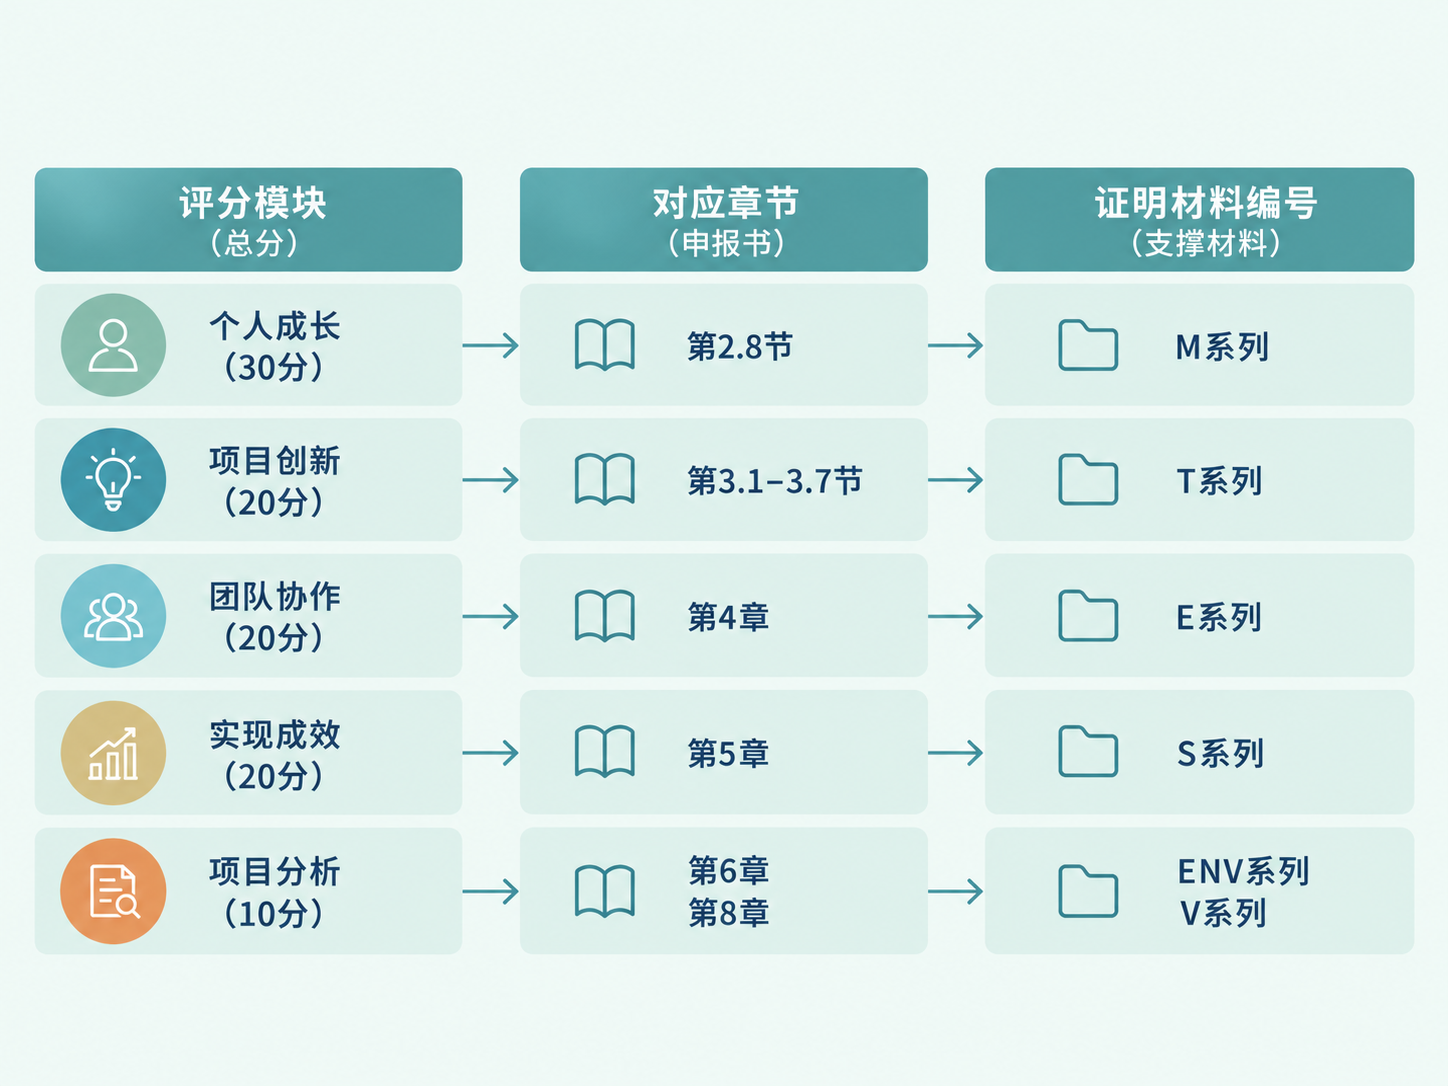
\includegraphics[width=\linewidth,height=.50\textheight,keepaspectratio]{figures/updated-1-1.png}
\caption{评分标准、计划书位置与证据编号对应图}\label{fig:1-1}
\par\vspace{3pt}{\fontsize{9}{12}\selectfont\linespread{1}\selectfont 注：本图为所供图稿的概览示意，部分章节与编号连线采用简化表达。个人成长对应 M/\allowbreak{}T/\allowbreak{}E/\allowbreak{}V 系列，团队协作对应第 8.1 节，实现成效对应第 2.3 节、第 5 章及第 6 章，项目分析对应第 4 章；完整对应关系以表 1-1 为准。}
\end{figure}
